%%%%%%%%%%%%%%%%%%%%%%%%%%%%%%%%%%%%%%%%%%%%%%%%%%%
% CHƯƠNG 3: THIẾT KẾ VÀ CHẾ TẠO PHẦN CỨNG THIẾT BỊ
%%%%%%%%%%%%%%%%%%%%%%%%%%%%%%%%%%%%%%%%%%%%%%%%%%%
\section*{CHƯƠNG 3. THIẾT KẾ VÀ CHẾ TẠO PHẦN CỨNG THIẾT BỊ}
\addcontentsline{toc}{section}{\numberline{}CHƯƠNG 3. THIẾT KẾ VÀ CHẾ TẠO PHẦN CỨNG THIẾT BỊ}
\setcounter{section}{3}
\setcounter{subsection}{0}
\setcounter{figure}{0}
\setcounter{table}{0}

\subsection{Sơ đồ khối hệ thống phần cứng}
Hệ thống phần cứng đeo tay được xây dựng bao gồm 7 khối chức năng liên kết chặt chẽ với nhau như mô tả trong sơ đồ khối Hình \ref{fig:block_diagram}:
\begin{itemize}
    \item \textbf{Cổng kết nối USB Type-C:} Đầu ngõ tiếp nhận nguồn sạc 5V và kết nối các đường truyền tín hiệu gỡ lỗi/nạp chương trình trực tiếp.
    \item \textbf{Khối nguồn sạc pin:} Nhận nguồn 5V từ cổng USB Type-C sạc cho pin Lithium 3.7V qua IC TP4056 và tích hợp mạch bảo vệ an toàn DW01A.
    \item \textbf{Khối ổn áp LDO hạ áp:} Hạ điện áp pin Lithium xuống 3.3V ổn định cấp cho MCU và các ngoại vi qua IC AMS1117-3.3V.
    \item \textbf{Khối vi điều khiển trung tâm:} SoC ESP32-C3 chịu trách nhiệm đọc dữ liệu cảm biến, chạy thuật toán lọc số DSP và phát Wi-Fi.
    \item \textbf{Khối cảm biến sinh hiệu:} MAX30102 đo PPG và HDC2022 đo nhiệt ẩm cơ thể, kết nối qua bus truyền thông I2C.
    \item \textbf{Khối hiển thị cục bộ:} OLED SSD1306 hiển thị thông số và trạng thái kết nối mạng tại chỗ.
    \item \textbf{Khối phím bấm vật lý:} Các nút nhấn điều khiển và cấu hình phần cứng (MODE, RESET, BOOT) kết nối trực tiếp đến GPIO của vi điều khiển.
\end{itemize}

\begin{figure}[H]
    \centering
    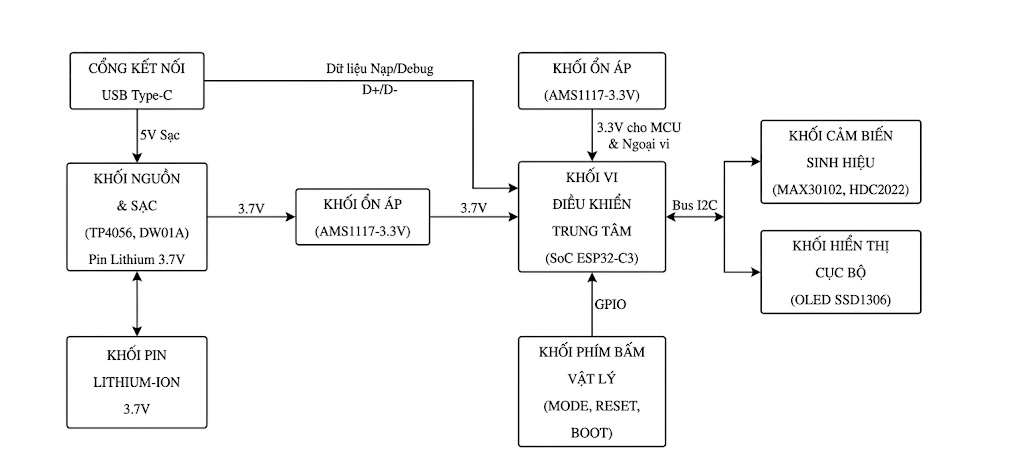
\includegraphics[width=\textwidth]{images/hardware/sodo_khoi.png}
    \caption[Sơ đồ khối chức năng chi tiết của thiết bị phần cứng đeo tay]{\bfseries\fontsize{12pt}{0pt}\selectfont Sơ đồ khối chức năng chi tiết của thiết bị phần cứng đeo tay}
    \label{fig:block_diagram}
\end{figure}

\subsection{Thiết kế sơ đồ nguyên lý}
Sơ đồ nguyên lý toàn mạch được thiết kế trên phần mềm Altium Designer bao gồm các khối chức năng chính như mô tả trong Hình \ref{fig:altium_schematic_total}:

\begin{figure}[H]
    \centering
    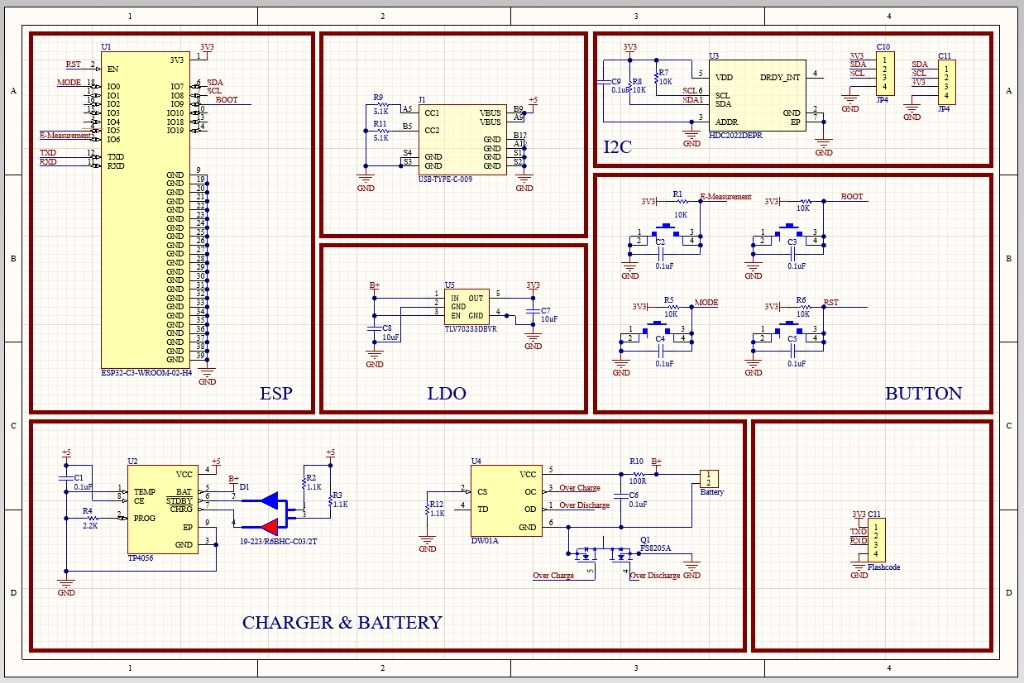
\includegraphics[width=0.95\textwidth]{images/hardware/schematic.jpg}
    \caption[Sơ đồ nguyên lý thiết kế toàn mạch của thiết bị đeo]{\bfseries\fontsize{12pt}{0pt}\selectfont Sơ đồ nguyên lý thiết kế toàn mạch của thiết bị đeo}
    \label{fig:altium_schematic_total}
\end{figure}

\subsubsection{Khối nguồn}
Nguồn điện sạc 5V từ cổng USB Type-C đi qua cầu chì tự phục hồi PPTC dòng giữ 500mA để bảo vệ quá dòng đầu vào. Điện áp 5V cấp vào chân VCC (chân 4) của IC TP4056. Chân PROG (chân 2) được kết nối một điện trở xuống GND để xác lập dòng sạc pin cực đại:
\begin{equation}
    I_{\text{charge}} = \frac{1000}{R_{\text{prog}}} = \frac{1000}{2.4\text{k}\Omega} \approx 416\text{mA}
\end{equation}
Dòng sạc này hoàn toàn nằm trong giới hạn an toàn của pin Lithium 3.7V dung lượng 500mAh (giới hạn sạc dòng 0.8C). Để bảo vệ pin chuyên sâu, em kết nối cực âm của pin sạc với cực máng của Mosfet FS8205A. IC bảo vệ DW01A liên tục đo điện áp giữa chân VDD và VSS của pin:
\begin{itemize}
    \item Nếu điện áp pin vượt quá 4.3V, DW01A ngắt chân OC ngắt Mosfet sạc để bảo vệ chống quá sạc.
    \item Nếu điện áp pin giảm dưới 2.4V, DW01A ngắt chân OD ngắt Mosfet xả để bảo vệ chống xả kiệt gây chai pin.
    \item Nếu dòng điện xả quá lớn (chập tải đầu ra), DW01A ngắt chân OD lập tức trong vài micro giây để chống cháy nổ.
\end{itemize}

\subsubsection{Khối vi điều khiển}
Mô-đun ESP32-C3-WROOM-02 nhận điện áp 3.3V cấp vào chân VDD. Để lọc nhiễu tần số cao cho đường nguồn của MCU, em bố trí hai tụ gốm $10\mu\text{F}$ và $100\text{nF}$ đặt sát chân nguồn VDD của mô-đun. Chân khôi phục phần cứng EN được kéo lên nguồn 3.3V thông qua điện trở $10\text{k}\Omega$ và tụ hóa $1\mu\text{F}$ nối đất để tạo thời gian trễ ổn định nguồn khi bắt đầu khởi động. Chân GPIO9 được kéo lên mức cao bằng điện trở $10\text{k}\Omega$ để đảm bảo MCU luôn boot vào chế độ chạy code từ bộ nhớ Flash khi khởi động thông thường.

\subsubsection{Khối cảm biến}
Khối cảm biến thu thập các thông số sinh hiệu bao gồm cảm biến quang học MAX30102 để đo nhịp tim và $SpO_2$, cùng cảm biến nhiệt độ kỹ thuật số HDC2022 để đo nhiệt độ da và độ ẩm môi trường. Cả hai cảm biến này đều giao tiếp với vi điều khiển ESP32-C3 thông qua bus I2C sử dụng hai chân GPIO7 (SDA) và GPIO8 (SCL). Hai đường bus này được kéo lên nguồn điện áp 3.3V thông qua cặp điện trở kéo lên $R_1 = R_2 = 4.7\text{k}\Omega$ để triệt tiêu điện dung ký sinh đường truyền, đảm bảo truyền dữ liệu ổn định ở tần số hoạt động 400kHz.

\subsubsection{Khối hiển thị}
Màn hình OLED SSD1306 1.3 inch được sử dụng để hiển thị trực quan các thông số sinh hiệu đo đạc được tại chỗ. Màn hình kết nối với vi điều khiển qua bus I2C chung với khối cảm biến (sử dụng chân GPIO7 và GPIO8). Nhờ địa chỉ I2C khác biệt của từng thiết bị ngoại vi, vi điều khiển có thể gửi dữ liệu hiển thị lên OLED một cách chính xác mà không gây xung đột tín hiệu trên đường truyền.

\subsubsection{Khối nạp chương trình}
Để tối ưu không gian phần cứng cho thiết bị đeo tay nhỏ gọn, thiết bị không sử dụng chip chuyển đổi USB-to-UART ngoại vi (như CH340C). Thay vào đó, em tận dụng bộ điều khiển USB Serial/JTAG Controller tích hợp sẵn bên trong SoC ESP32-C3. Các chân truyền dữ liệu của cổng USB Type-C (D+ và D-) được nối thẳng tới chân GPIO19 (D+) và GPIO18 (D-) của ESP32-C3. Máy tính có thể nhận dạng vi điều khiển trực tiếp dưới dạng một cổng COM ảo để nạp code và debug chương trình mà không cần chip nạp phụ. Quá trình nạp code được điều khiển hoàn toàn bằng nút bấm vật lý.

\subsubsection{Khối nút bấm}
Để phục vụ quá trình điều khiển và nạp chương trình thủ công, thiết bị được thiết kế với 3 nút bấm vật lý chuyên dụng:
\begin{itemize}
    \item \textbf{Nút BOOT}: Kết nối trực tiếp vào chân cấu hình boot GPIO9 của vi điều khiển ESP32-C3. Khi nhấn nút, chân GPIO9 được kéo xuống mức thấp (GND).
    \item \textbf{Nút RESET}: Kết nối vào chân reset EN của vi điều khiển. Khi nhấn nút, chân EN được kéo xuống mức thấp, buộc vi điều khiển khởi động lại phần cứng.
    \item \textbf{Nút MODE}: Kết nối vào chân GPIO0 để phục vụ chuyển đổi các chế độ hoạt động hoặc giao diện hiển thị của thiết bị đeo tay.
\end{itemize}
Để đưa vi điều khiển ESP32-C3 vào chế độ Bootloader sẵn sàng nạp chương trình mới từ máy tính, quy trình nhấn nút vật lý thủ công được thực hiện như sau:
\begin{enumerate}
    \item Nhấn giữ nút BOOT để giữ chân GPIO9 ở mức thấp.
    \item Nhấn rồi thả nút RESET để khởi động lại chip trong khi chân GPIO9 vẫn ở mức thấp.
    \item Thả nút BOOT. Lúc này vi điều khiển sẽ khởi động vào ROM Bootloader để chờ nhận file nạp từ phần mềm esptool.
\end{enumerate}

\begin{figure}[H]
    \centering
    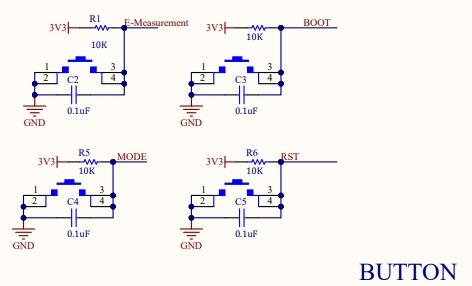
\includegraphics[width=0.6\textwidth]{images/hardware/schematic_button.jpg}
    \caption[Sơ đồ nguyên lý mạch nút bấm điều khiển và mạch reset]{\bfseries\fontsize{12pt}{0pt}\selectfont Sơ đồ nguyên lý mạch nút bấm điều khiển và mạch reset}
    \label{fig:schematic_button}
\end{figure}

\subsection{Quy trình thiết kế mạch in PCB và mô hình 3D}
Bo mạch in được layout 2 lớp (2-layer) trên phần mềm Altium Designer với độ dày phíp đồng tiêu chuẩn 1.6mm. Biên dạng mạch in được cắt vát dạng bát giác đều nhỏ gọn có kích thước phủ bì 42x42mm để lắp vừa khuôn vỏ đồng hồ đeo tay. Bản vẽ thiết kế đường mạch in lớp Top (mặt trên) và lớp Bottom (mặt dưới) được thể hiện chi tiết tại Hình \ref{fig:altium_pcb_layout}.

\begin{figure}[H]
    \centering
    \begin{minipage}{0.48\textwidth}
        \centering
        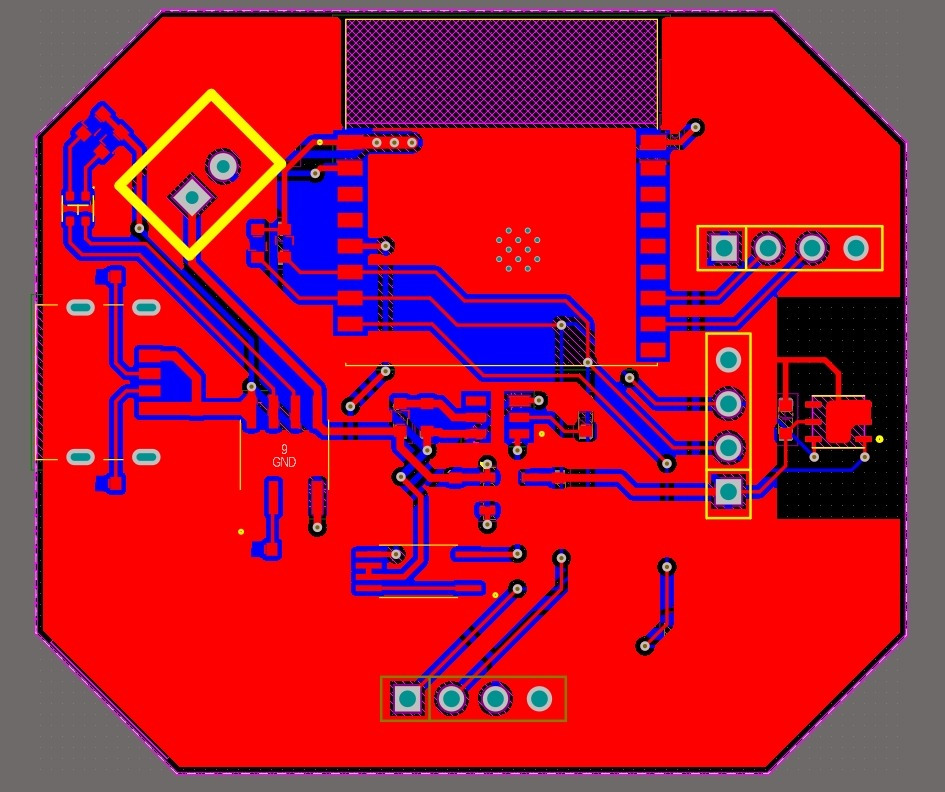
\includegraphics[width=\textwidth]{images/hardware/pcb_layout_top.jpg}
        \centerline{a) Lớp Top (đường đi dây mặt trên)}
    \end{minipage}
    \hfill
    \begin{minipage}{0.48\textwidth}
        \centering
        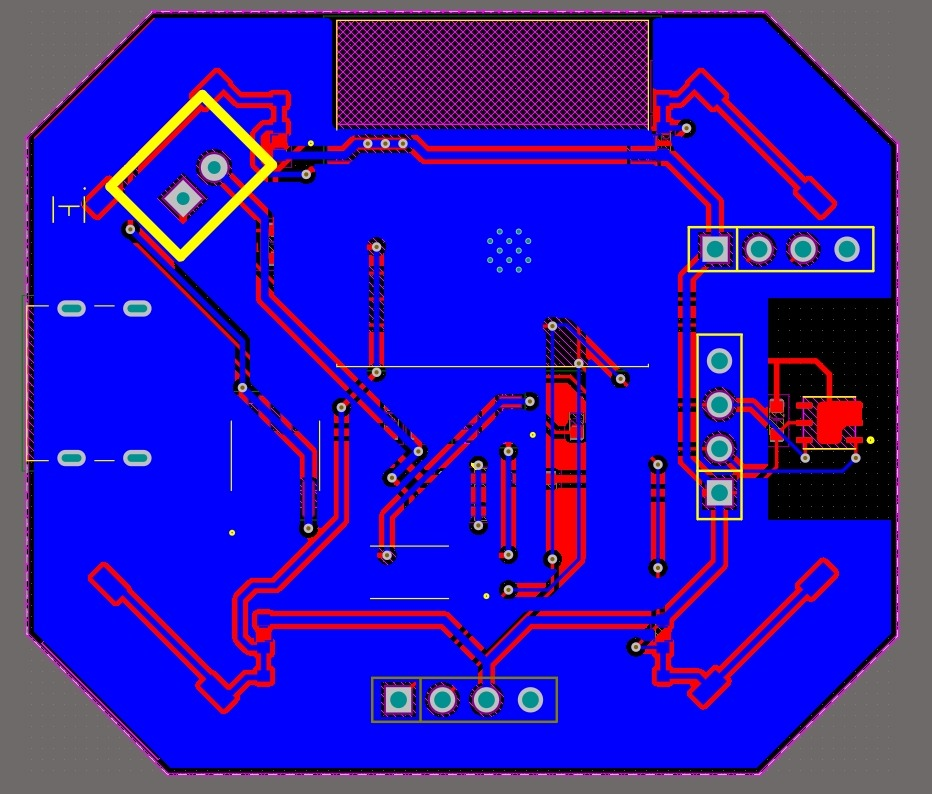
\includegraphics[width=\textwidth]{images/hardware/pcb_layout_bottom.jpg}
        \centerline{b) Lớp Bottom (đường đi dây mặt dưới)}
    \end{minipage}
    \caption[Bản vẽ thiết kế đường đi dây trên bo mạch in PCB]{\bfseries\fontsize{12pt}{0pt}\selectfont Bản vẽ thiết kế đường đi dây trên bo mạch in PCB}
    \label{fig:altium_pcb_layout}
\end{figure}

Các nguyên tắc thiết kế mạch in tần số cao được áp dụng nghiêm ngặt:
\begin{itemize}
    \item \textbf{Đi dây nguồn dòng lớn:} Đường mạch nguồn chính 5V và 3.3V đi dây kích thước lớn 24mil để tránh hiện tượng sụt áp đường dây khi mô-đun Wi-Fi của ESP32-C3 hoạt động phát sóng công suất lớn đột ngột.
    \item \textbf{Thiết kế bus tín hiệu số:} Các đường truyền bus dữ liệu SDA, SCL đi dây kích thước 8mil, chạy song song sát nhau và có chiều dài bằng nhau để hạn chế lệch pha tín hiệu.
    \item \textbf{Kỹ thuật bọc mass chống nhiễu cảm biến:} Vùng mạch Analog nhạy cảm của cảm biến quang học MAX30102 được bọc cách ly bởi đường phủ đồng mass tiếp địa (GND Pour) riêng biệt và đi xa vùng anten phát sóng RF Wi-Fi của vi điều khiển ESP32-C3 để ngăn nhiễu trường điện từ vô tuyến RF xâm nhập vào kênh đọc dòng cực nhỏ (nA) của đi-ốt quang.
\end{itemize}

Mô hình thiết kế 3D hoàn chỉnh của bo mạch sau khi layout được dựng trực tiếp trên Altium Designer mặt trước và mặt sau như mô tả ở Hình \ref{fig:altium_pcb_3d}.

\begin{figure}[H]
    \centering
    \begin{minipage}{0.48\textwidth}
        \centering
        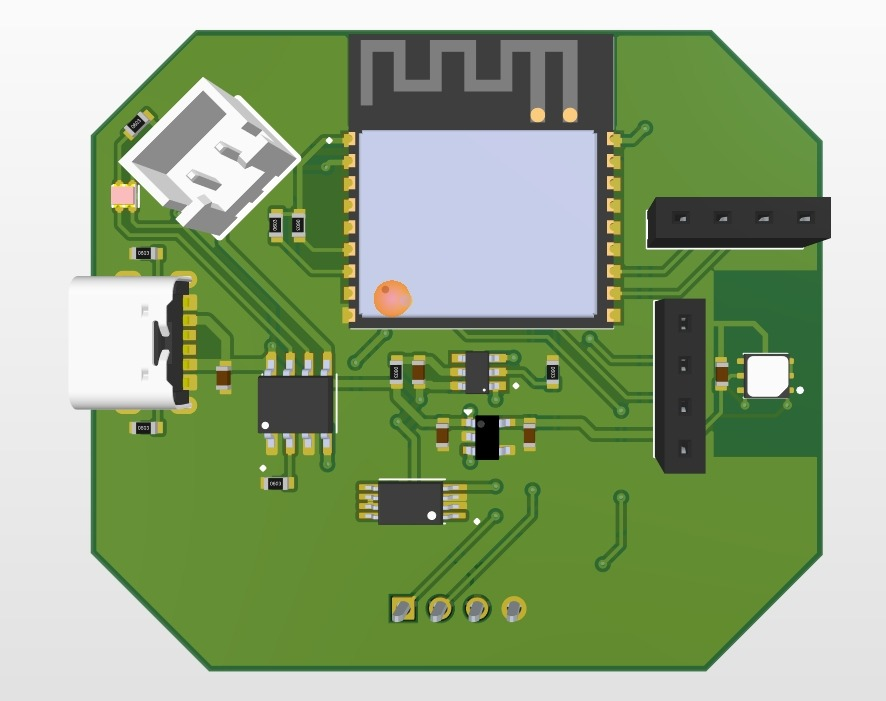
\includegraphics[width=\textwidth]{images/hardware/pcb_3d_top.jpg}
        \centerline{a) Mặt trước (Top View)}
    \end{minipage}
    \hfill
    \begin{minipage}{0.48\textwidth}
        \centering
        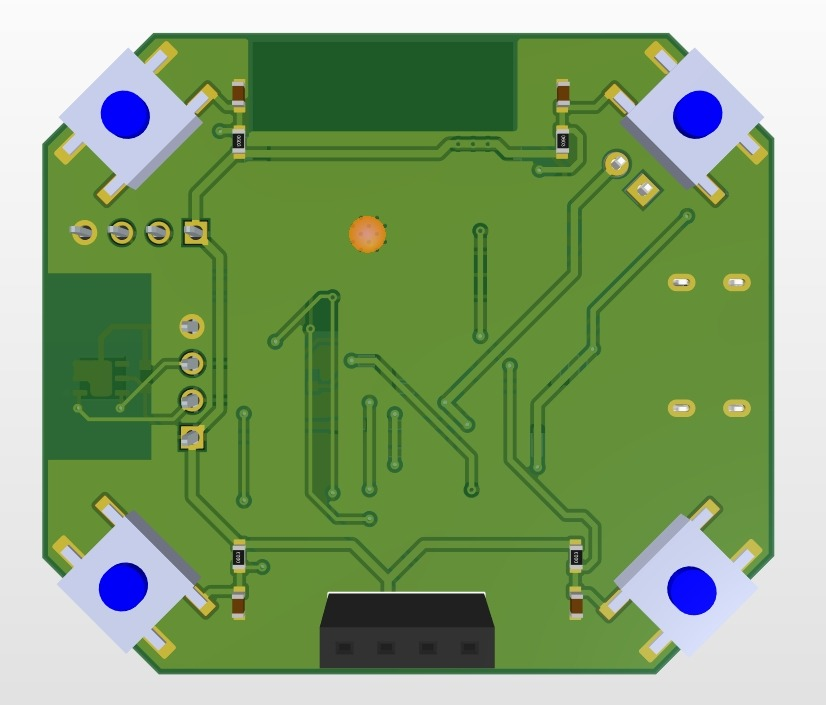
\includegraphics[width=\textwidth]{images/hardware/pcb_3d_bottom.jpg}
        \centerline{b) Mặt sau (Bottom View)}
    \end{minipage}
    \caption[Mô hình mô phỏng 3D hoàn chỉnh của bo mạch thiết bị đeo]{\bfseries\fontsize{12pt}{0pt}\selectfont Mô hình mô phỏng 3D hoàn chỉnh của bo mạch thiết bị đeo}
    \label{fig:altium_pcb_3d}
\end{figure}
